\documentclass[../main.tex]{subfiles}
\begin{document}
\paragraph{Simulation 3}\label{par:sim_3}

\begin{equation}\label{eq:sim_3_shift}
        g(s) \in \mathbb{P}_{9}[s]\,,\quad\{c_{1}=1.9,\, c_{2}=-0.6,\, c_{3}=-7,\, c_{4}=-2,\, c_{5}=1.7,\, c_{6}=2.4,\, c_{7}=3.2,\, c_{8}=0.4,\, c_{9}=2.2\}\,.
\end{equation}

\begin{figure}[H]
    \centering 
    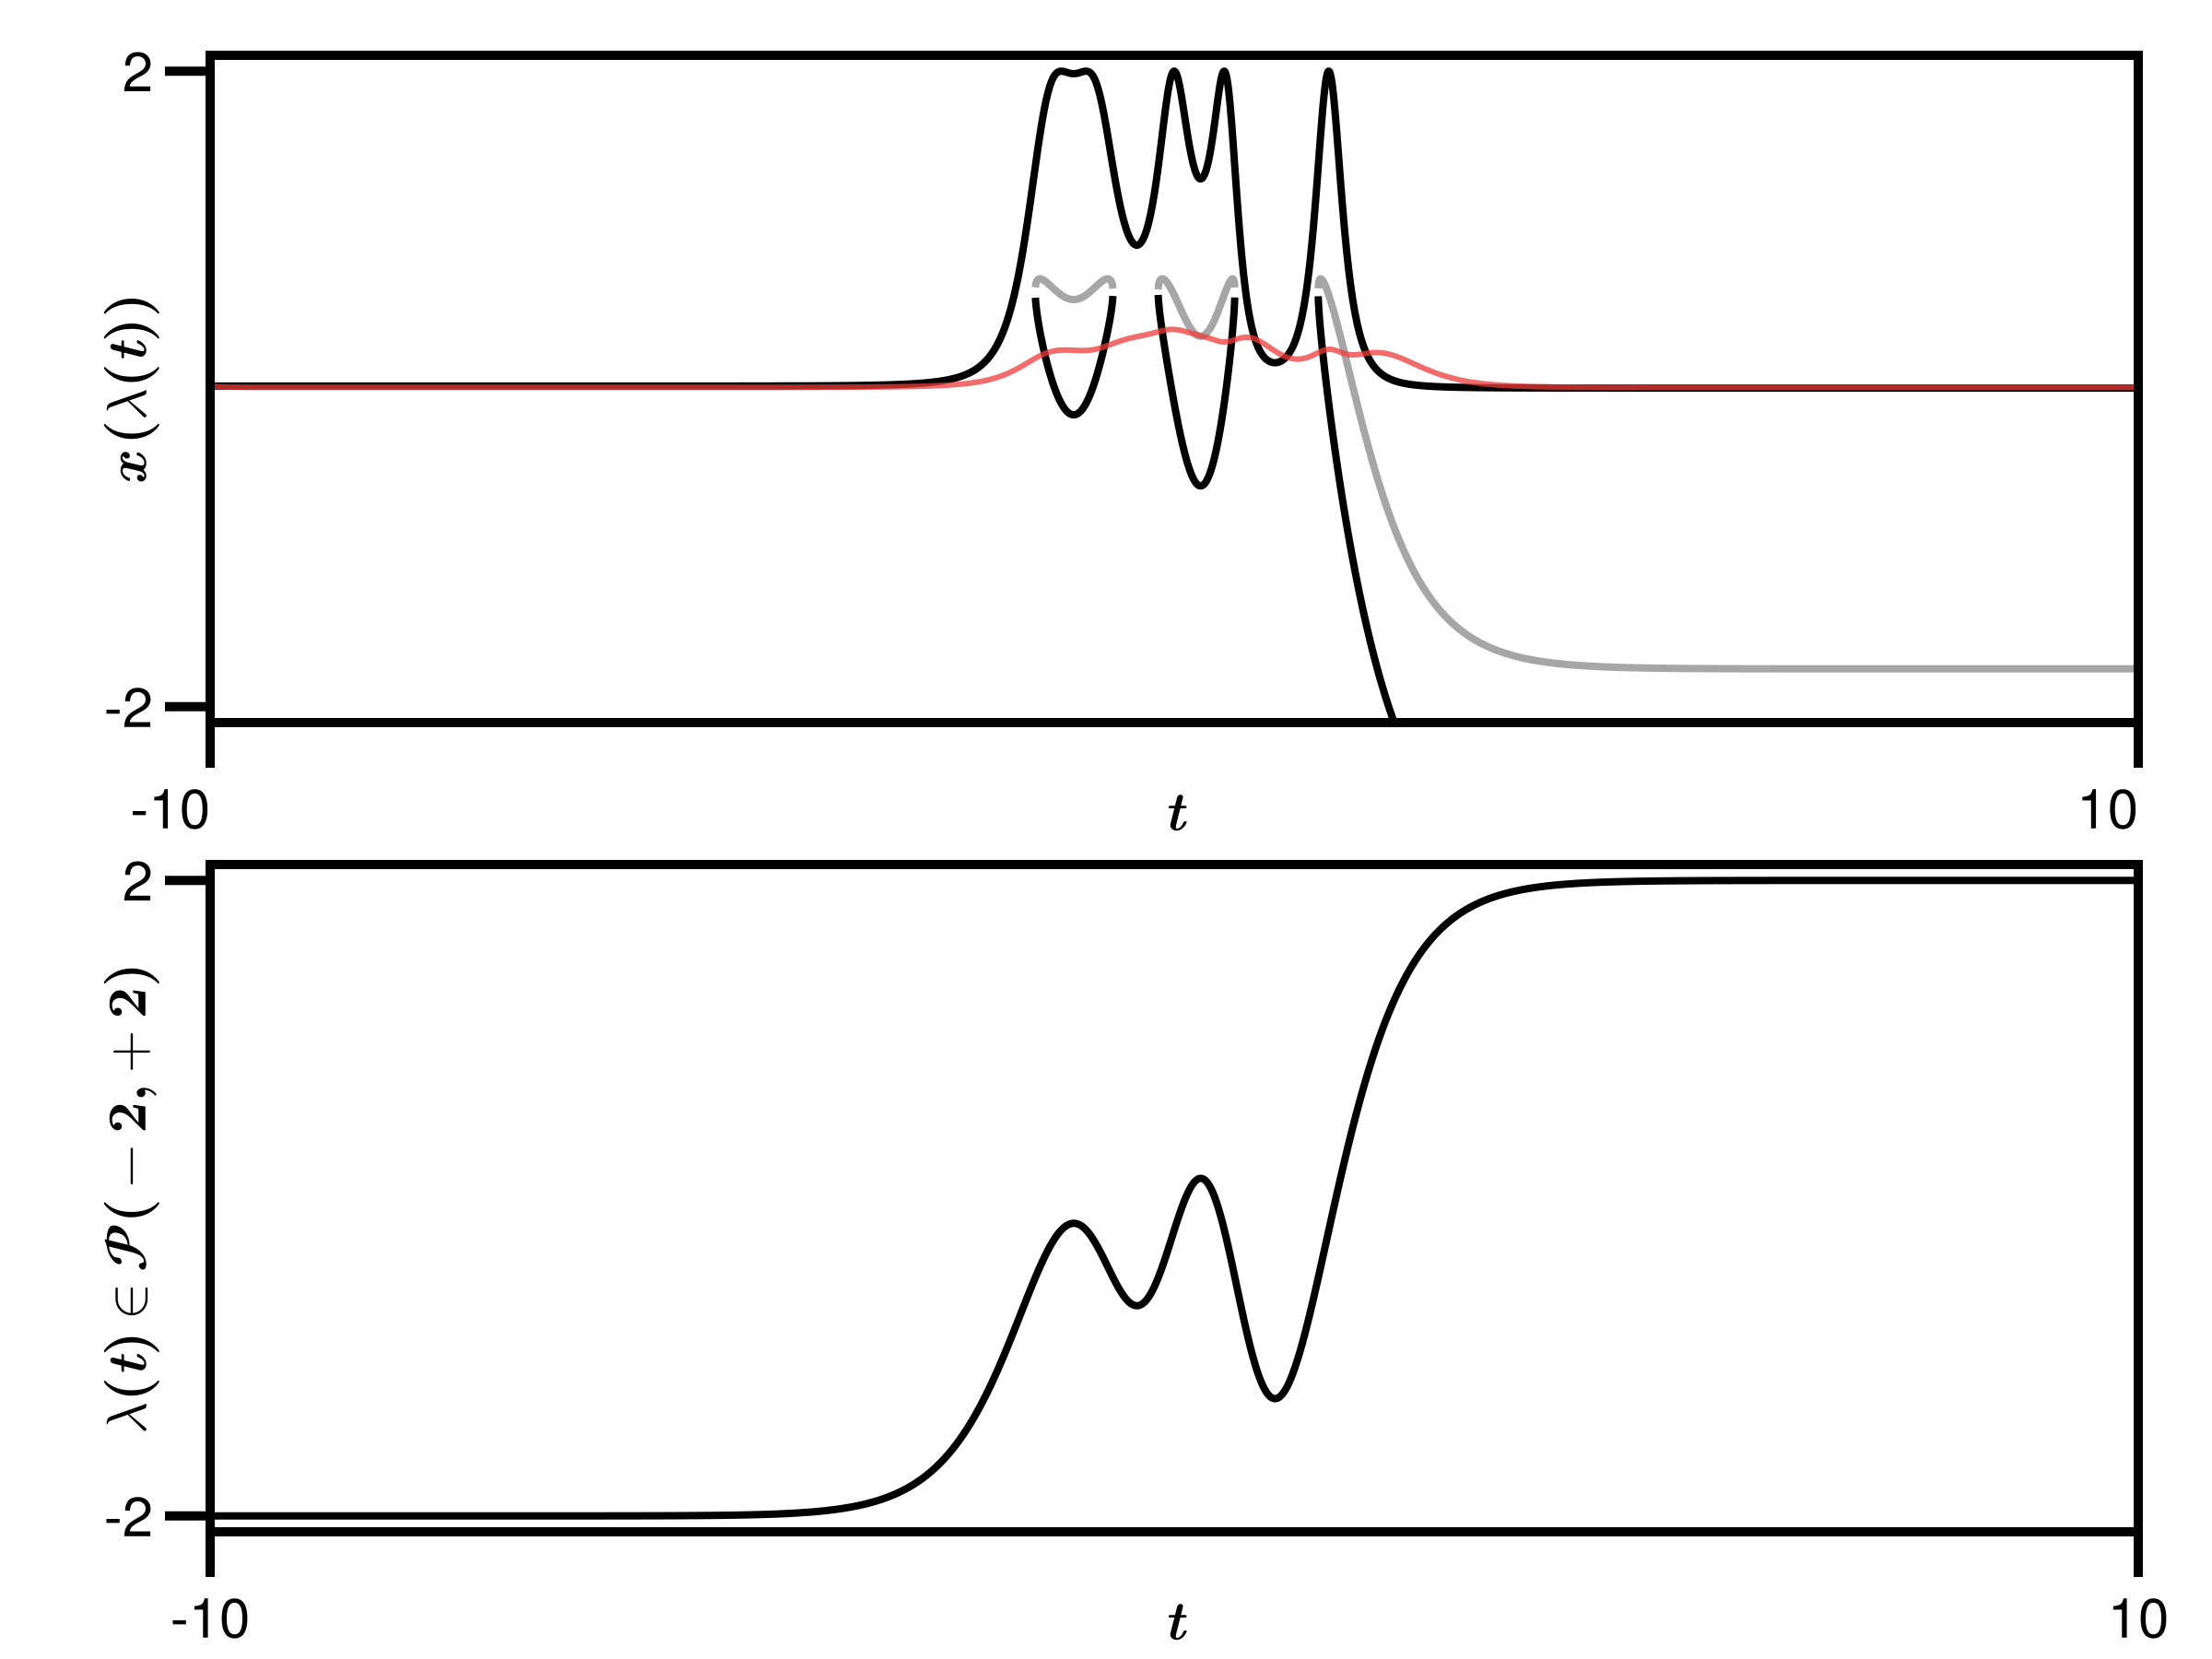
\includegraphics[keepaspectratio, width=\textwidth]{../figures/sim_3.png}
    \caption{Solution of \eqref{eq:dyn_sys} (top) with the parameter shift \eqref{eq:sim_3_shift} (bottom). No R-tipping.}
    \label{fig:sim_3}
\end{figure}

\end{document}
